\subsection{Gaussovský potenciál}
	Interakce je určena sféricky symetrickým potenciálem
	\begin{equation}
		V(r)=v\e^{-\mu r^{2}},
	\end{equation}
	kde $v$ a $\mu$ jsou reálné konstanty, $\mu>0$.
	
	\begin{enumerate}
	\item 
		Určete v Bornově aproximaci amplitudu rozptylu a diferenciální účinný průřez rozptylu na tomto potenciálu.
		
	\item 
		Určete fázové posunutí pro $s$ vlnu.
				
	\item
		Určete fázové posunutí pro $p$ vlnu.
	\end{enumerate}
	
\begin{solution}
	Předně označíme $\vector{q}=\vector{k}-\vector{k}'$ a úhel mezi vektory $\vector{k}$ a $\vector{k'}$ jako $\psi$.
	Pak (díky rovnosti velikostí vlnových vektorů $k=k'$)
	\begin{equation}
		q^{2}=k^{2}-2\vector{k}\cdot\vector{k}'+k^{'2}=2k^{2}\left(1-\cos{\psi}\right)=4k^{2}\sin^{2}\frac{\psi}{2},
	\end{equation}
	a tedy
	\begin{equation}
		q=2k\sin{\frac{\psi}{2}}.
	\end{equation}

	\begin{enumerate}
		\item
			Amplituda rozptylu se spočítá přímočaře pomocí vzorce~\eqref{eq:Born}:
			\begin{align}
				f(\vector{k}',\vector{k})
					&=-\frac{Mv}{2\pi\hbar^{2}}\int\e^{\im\vector{q}\cdot\vector{r}}\e^{-\mu r^{2}}\d^{3}\vector{r}=\equationcomment{\text{sférické souřadnice,}\\\text{osa }z\text{ paralelní s }\vector{q}\\\vector{q}\cdot\vector{r}=qr\cos{\theta}}\nonumber\\
					&=-\frac{Mv}{2\pi\hbar^{2}}\int_{0}^{\infty}\int_{0}^{\pi}\int_{0}^{2\pi}\e^{\im qr\cos{\theta}}\e^{-\mu r^{2}}r^{2}\sin{\theta}\,\d r\,\d\theta\,\d\phi
					 =\equationcomment{u=\cos{\theta}\\ \d u=-\sin{\theta}\,\d\theta}\nonumber\\
					&=-\frac{Mv}{\hbar^{2}}\int_{0}^{\infty}r^{2}\e^{-\mu r^{2}}\,\d r\int_{-1}^{1}\e^{\im qru}\,\d u\nonumber\\
					&=-\frac{Mv}{\hbar^{2}}\int_{0}^{\infty}r^{2}\e^{-\mu r^{2}}\left[\frac{\e^{\im qru}}{\im qr}\right]_{-1}^{1}\d r
					 =-\frac{Mv}{\im q\hbar^{2}}\int_{0}^{\infty}\left(\e^{-\mu r^{2}+\im qr}-\e^{-\mu r^{2}-\im qr}\right)r\,\d r\nonumber\\
					&=-\frac{Mv}{\im q\hbar^{2}}\e^{-\frac{q^{2}}{4\mu}}\int_{0}^{\infty}\left[\e^{-\mu\left(r-\frac{\im q}{2\mu}\right)^{2}}-\e^{-\mu\left(r+\frac{\im q}{2\mu}\right)^{2}}\right]r\,\d r
					 =\equationcomment{x=r-a \\ y=r+a \\ a=\frac{\im q}{2\mu}}\nonumber\\
					&=-\frac{Mv}{\im q\hbar^{2}}\e^{-\frac{q^{2}}{4\mu}}\underbrace{\left[\int_{-a}^{\infty}\left(x+a\right)\e^{-\mu x^{2}}\d x-\int_{a}^{\infty}\left(y-a\right)\e^{-\mu y^{2}}\d y\right]}_{I}.
			\end{align}
			Integrál je
			\begin{align}
				I&=\int_{-a}^{0}x\e^{-\mu x^{2}}+a\int_{-a}^{0}\e^{-\mu x^{2}}\d x+\int_{0}^{\infty}x\e^{-\mu x^{2}}\d x+a\int_{0}^{\infty}\e^{-\mu x^{2}}\d x\nonumber\\
				 &\qquad-\int_{0}^{\infty}x\e^{-\mu x^{2}}\d x+a\int_{0}^{\infty}\e^{-\mu x^{2}}\d x+\int_{0}^{a}x\e^{-\mu x^{2}}\d x-a\int_{0}^{a}\e^{-\mu x^{2}}\d x\nonumber\\
				 &=2a\int_{0}^{\infty}\e^{-\mu x^{2}}\d x+\underbrace{\int_{-a}^{a}x\e^{-\mu x^{2}}\d x}_{0\text{ (lichá funkce)}}+\underbrace{a\int_{-a}^{0}\e^{-\mu x^{2}}\d x-a\int_{0}^{a}\e^{-\mu x^{2}}\d x}_{0\text{ (sudá funkce)}}\nonumber\\
				 &=2a\int_{0}^{\infty}\e^{-\mu x^{2}}\d x=a\sqrt{\frac{\pi}{\mu}},
			\end{align}
			takže amplituda rozptylu vychází
			\begin{equation}
				f(\vector{k}',\vector{k})=-\frac{Mv}{2\mu\hbar^{2}}\sqrt{\frac{\pi}{\mu}}\e^{-\frac{q^{2}}{4\mu}}
			\end{equation}
			a z ní diferenciální účinný průřez dle~\eqref{eq:ScatteringCrossSection}
			\begin{equation}
				\derivative{\sigma}{\Omega}=\frac{\pi (Mv)^{2}}{4\hbar^{4}\mu^{3}}\e^{-\frac{q^{2}}{2\mu}}.
			\end{equation}
			
		\item
			Amplituda rozptylu $s$-vlny ($l=0$) se vypočte pomocí vzorce~\eqref{eq:PartialScatteringAmplitudef}:
			\begin{align}
				f_{0}(k)
					&=-\frac{Mv}{4\mu\hbar^{2}}\sqrt{\frac{\pi}{\mu}}\int_{-1}^{1}\e^{-\frac{\overbrace{q^{2}}^{4k^{2}\sin^{2}\frac{\psi}{2}}}{4\mu}}\underbrace{P_{0}(\cos{\psi})}_{1}\,\d\cos{\psi}\nonumber\\
					&=-\frac{Mv}{4\mu\hbar^{2}}\sqrt{\frac{\pi}{\mu}}\int_{-1}^{1}\e^{-\frac{k^{2}}{2\mu}(1-x)}\d x\nonumber\\
					&=-\frac{Mv}{4\mu\hbar^{2}}\sqrt{\frac{\pi}{\mu}}\left[\frac{2\mu}{k^{2}}\e^{-\frac{k^{2}}{2\mu}(1-x)}\right]_{-1}^{1}\nonumber\\
					&=-\frac{Mv}{2\hbar^{2}k^{2}}\sqrt{\frac{\pi}{\mu}}\left(1-\e^{-\frac{k^{2}}{\mu}}\right)
					 =-\frac{Mv}{\hbar^{2}k^{2}}\sqrt{\frac{\pi}{\mu}}\e^{-\frac{k^{2}}{2\mu}}\sinh{\frac{k^{2}}{2\mu}}.
			\end{align}
			Fázové posunutí je pak na základě přibližného vzorce~\eqref{eq:PhaseShiftApprox} rovno
			\begin{equation}
				\delta_{0}(k)\approx-\frac{Mv}{\hbar^{2}k}\sqrt{\frac{\pi}{\mu}}\e^{-\frac{k^{2}}{2\mu}}\sinh{\frac{k^{2}}{2\mu}}.
			\end{equation}
		
		\item
			Aplituda rozptylu a fázové posunutí $p$-vlny se určí analogicky jako v předchozím bodě:
			\begin{align}
				f_{1}(k)
					&=-\frac{Mv}{4\mu\hbar^{2}}\sqrt{\frac{\pi}{\mu}}\int_{-1}^{1}\e^{-\frac{k^{2}}{2\mu}(1-x)}\underbrace{P_{1}(x)}_{x}\,\d x=\equationcomment{\text{Per partes}}\nonumber\\			
					&=-\frac{Mv}{4\mu\hbar^{2}}\sqrt{\frac{\pi}{\mu}}\left\{\left[\frac{2\mu}{k^{2}}x\e^{-\frac{k^{2}}{2\mu}(1-x)}\right]_{-1}^{1}-\frac{2\mu}{k^{2}}\int_{-1}^{1}\e^{-\frac{k^{2}}{2\mu}(1-x)}\,\d x\right\}\nonumber\\
					&=-\frac{Mv}{2\hbar^{2}k^{2}}\sqrt{\frac{\pi}{\mu}}\left\{1+\e^{-\frac{k^{2}}{\mu}}-\frac{2\mu}{k^{2}}\left(1-\e^{-\frac{k^{2}}{\mu}}\right)\right\}\nonumber\\
					&=-\frac{Mv}{2\hbar^{2}k^{2}}\sqrt{\frac{\pi}{\mu}}\e^{-\frac{k^{2}}{2\mu}}\left\{\left(\e^{\frac{k^{2}}{2\mu}}+\e^{-\frac{k^{2}}{2\mu}}\right)-\frac{2\mu}{k^{2}}\left(\e^{\frac{k^{2}}{2\mu}}-\e^{-\frac{k^{2}}{2\mu}}\right)\right\}\nonumber\\
					&=-\frac{Mv}{\hbar^{2}k^{2}}\sqrt{\frac{\pi}{\mu}}\e^{-\frac{k^{2}}{2\mu}}\left[\cosh{\frac{k^{2}}{2\mu}}-\frac{2\mu}{k^{2}}\sinh{\frac{k^{2}}{2\mu}}\right],\\
				\delta_{1}(k)
					&=-\frac{Mv}{\hbar^{2}k}\sqrt{\frac{\pi}{\mu}}\e^{-\frac{k^{2}}{2\mu}}\left[\cosh{\frac{k^{2}}{2\mu}}-\frac{2\mu}{k^{2}}\sinh{\frac{k^{2}}{2\mu}}\right].
			\end{align}		
	\end{enumerate}
	
	\begin{figure}[!hbp]
		\centering
			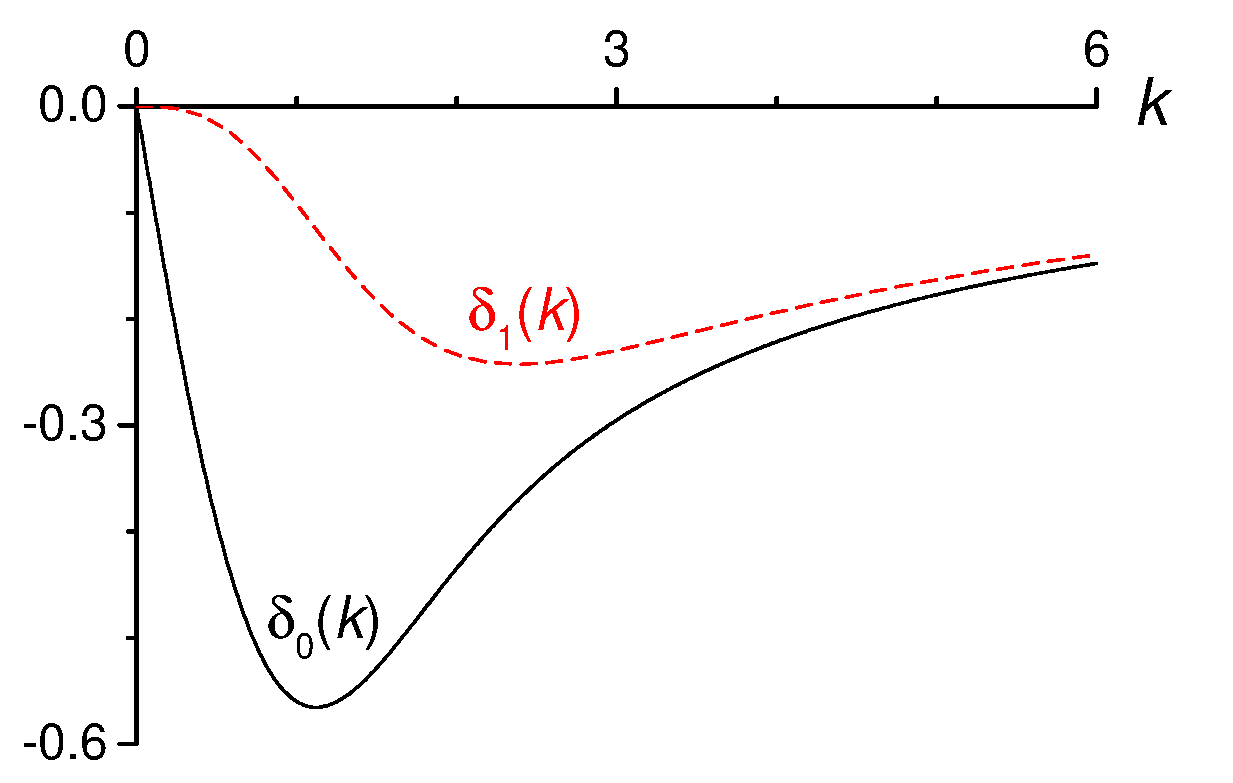
\epsfig{file=figures/gs.eps,width=0.6\linewidth,keepaspectratio}			
			\scaption{
				Fázová posunutí $s$ a $p$ parciální vlny pro rozptyl na Gaussovském potenciálu v 1. Bornově aproximaci.
				Hodnoty parametrů jsou $M=\hbar=v=\mu=1$.
			}	
        \label{fig:GaussianScattering}
	\end{figure}		
	
	Fázová posunutí pro $s$ a $p$ vlnu jsou znázorněna na obrázku~\ref{fig:GaussianScattering}.
\end{solution}